\documentclass[12pt,fullpage]{amsart}
\usepackage{graphicx,fullpage, multicol}

\input{/home/treisman/tex/macros}

%\input{/Users/treisman/tex/macros}
\graphicspath{{../../images/}}

\begin{document}

\simpletopofpage{Math 213}{ Practice Test \#3}{Fall 2021}

\begin{enumerate}

 \item
Ebay sellers wonder if the type of photo posted with an item affects the selling price of that item.  One hundred and forty three MarioKart packages were analyzed, which were classified as having a ``stock'' photo or not.  A $t$ distribution is used to compute a 95\% confidence interval for the average difference in selling price between those without and with ``stock'' photos ($\mu_{no}-\mu_{yes}$) is (-\$7.20, -\$1.14).  Which of the following are \underline{correct} interpretations of this interval?
\begin{enumerate}
    \item
    There is no evidence that photo type is associated selling price.
    \item
    We have evidence that packages with stock photos sell, on average, for more than packages without stock photos.
    \item
    We have evidence that packages with stock photos sell, on average, for less than packages without stock photos.
    \item
    In general, the average selling price of the MarioKart packages is less than \$10.
    \item
    More than one statement is correct.  
\end{enumerate}

\vfill

\item A researcher plans to study levels of Seasonal Affective Disorder in the Gunnison Valley. He recruits 30 people for his study and collects survey data from each of them twice, once in summer and once in winter. From each survey, he computes a happiness index, which is a number on a continuous scale between 0 and 1, with 0 indicating severe unhappiness and 1 indicating complete happiness. Which of the following procedures would be most appropriate for analyzing the relationship between season and happiness index?

  \begin{enumerate}
  \item Analysis of variance
  \item Linear regression
  \item Two sample t test
  \item Paired data t test
    \item None of the above are appropriate.
  \end{enumerate}

\vfill
  
  \newpage
  
\item Road tests of 32 cars\footnote{These data were published by Motor Trend magazine in 1974, analysed in \emph{Henderson and Velleman (1981), Building multiple regression models interactively. Biometrics, 37, 391-411} and are included in R as part of the \texttt{mtcars} dataset.} produced data about the relationship between horsepower and gas mileage. The output of a linear model is shown. A scatterplot with the fitted line from the linear model, as well as a histogram of the residuals and scatterplot of the residuals compared to the input variable.
\begin{verbatim}
Coefficients:
            Estimate Std. Error t value Pr(>|t|)    
(Intercept) 30.09886    1.63392  18.421  <0.0001 ***
cars$hp     -0.06823    0.01012  -6.742  <0.0001 ***
\end{verbatim}

\begin{center}
  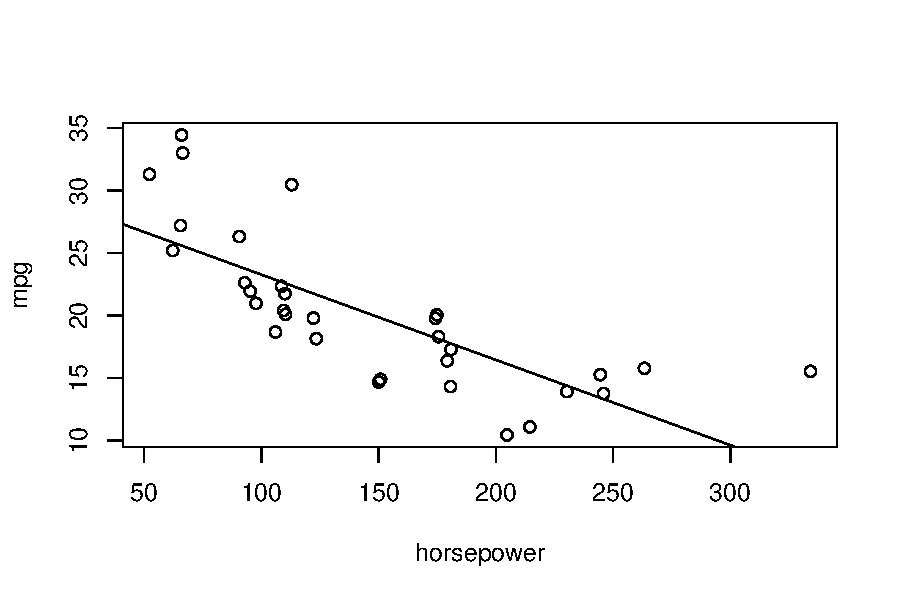
\includegraphics[width=10cm]{cars}\\
  \includegraphics[width=7cm]{hpmpgResiduals}\quad
  \includegraphics[width=7cm]{hpmpgResHist}
\end{center}

  \begin{enumerate}
  \item What was the null hypotheses tested for the \texttt{cars\$hp} coefficient?

  \item What can you conclude about the relationship between horsepower and gas mileage?

\item Do the assumptions that underlie linear regression appear satisfied by this model? Explain.

  \end{enumerate}

  \vfill
  
\item The same data set also contains the number of cylinders for each car and the time in seconds for each car to travel a quarter mile, starting from a stop, in seconds. Here are relevant data and graphics for analyzing the relationship between quarter mile times and number of cylinders:
  
\begin{tabular}{c|ccc}
cylinders& mean & sd & n\\
\hline
4 & 19.1 & 1.7 & 11\\
6 & 18.0 & 1.7 & 7\\
8 & 16.8 & 1.2 & 14
\end{tabular}

\begin{center}
\includegraphics[width=6cm]{4cylqsec}\quad
\includegraphics[width=6cm]{6cylqsec}\quad
\includegraphics[width=6cm]{8cylqsec}
\end{center}

  \begin{enumerate}
  \item One of the conditions for ANOVA appears questionable for these data. What is this condition, and why is it in question?
  \item ANOVA is somewhat robust in regards this condition. Here is the result of running ANOVA for quarter mile times in terms of cylinders.
\begin{verbatim}
          Df Sum Sq Mean Sq F value   Pr(>F)   
cars$cyl   2 34.606 17.3029  7.7938 0.001955 **
Residuals 29 64.382  2.2201    
\end{verbatim}
At the $\alpha=0.05$ significance level, does this indicate a difference between quarter mile times for cars with different numbers of cylinders?
\item A significant result from ANOVA leads to testing each pair of groups to determine which differences are significant. The following output lists the comparison performed, the expected difference in group means, a 95\% confidence interval for those differences, and a p value for a test of no difference.
\begin{verbatim}
comparison difference lower     upper      p adj
6-4        -1.16013   -2.939271  0.6190113  0.2574564
8-4        -2.36513   -3.847748 -0.8825122  0.0013300
8-6        -1.20500   -2.908398  0.4983980  0.2053353
\end{verbatim}
According to this output, is there a difference between quarter mile times between cars with 6 cylinder and 4 cylinder engines? Between 8 cylinder and 4 cylinder engines? Between 8 cylinder and 6 cylinder engines?
  \end{enumerate}

\vfill
  
\item In a study on Monarch butterflies, the relationship between wing weight in milligrams and wing area in square millimeters is plotted. A scatterplot of the data along with a linear regression line
  are shown below.  This line has equation $y = 395.01 + 38.23 x$ and
  correlation coefficient $R=0.802$
  \begin{enumerate}
  \item What is the biological meaning of the intercept 395.01?  Do
    you trust this?  Why or why not?

  \item What is the biological meaning of the slope 38.23?  Do
    you trust this?  Why or why not?

    \item What information does the correlation coefficient 0.802 provide?

  \item What do you expect that the area of a wing weighing 8 milligrams to be?

  \end{enumerate}
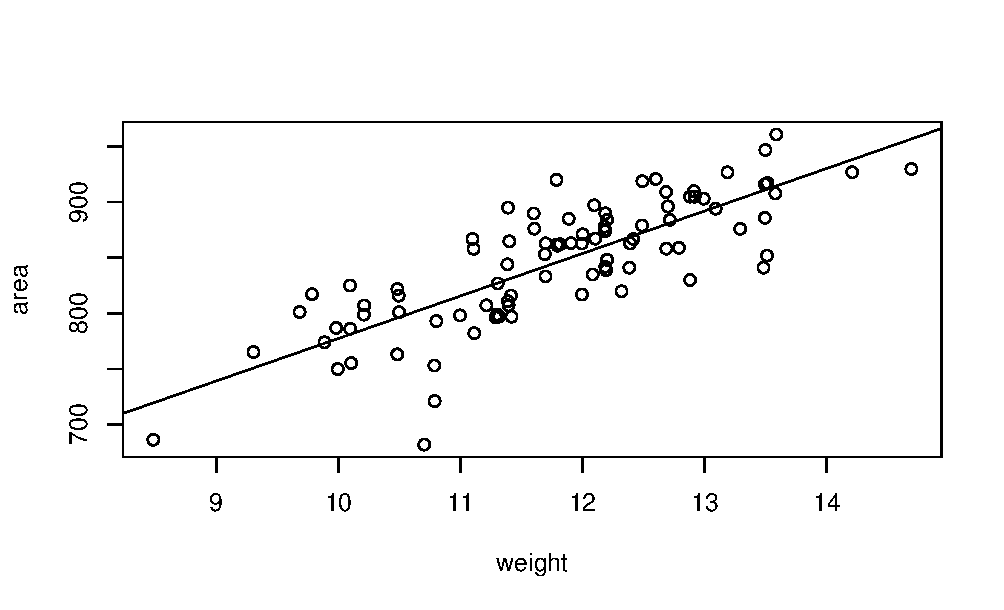
\includegraphics[scale=0.7]{areaWeight}

\end{enumerate} 

\end{document}
